\documentclass{article}
% \usepackage[showframe]{geometry}
\usepackage[hmarginratio=2:3, width=30pc]{geometry}
\usepackage{amsfonts, amssymb, amsmath}
\usepackage{multirow}
\usepackage{tikz}
\usetikzlibrary{positioning} % venn library can be useful, but drawing manually offers more control for labeling areas

\usepackage{subcaption}
\usepackage{graphicx}
\usepackage{float}
\usepackage{mdframed}
\usepackage[dvipsnames]{xcolor}

\definecolor{formulaShade}{RGB}{255,250,240}

\newmdenv[
  backgroundcolor=formulaShade,
  linecolor=gray,
  linewidth=0.8pt,
  roundcorner=4pt,
  innertopmargin=6pt,
  innerbottommargin=6pt,
  skipabove=10pt,
  skipbelow=10pt
]{FormulaBox}

\usepackage{hyperref}
\usepackage{lmodern}
% \usepackage{amsmath} % Required for \text, etc.
% \usepackage{amsfonts} % Required for math symbols
% \usepackage{amssymb} % Required for math symbols
\usepackage{array}   % Required for extra column formatting like >{\centering\arraybackslash}m{...}
\usepackage{xfrac}
%
% For alternative styles, see the biblatex manual:
% http://mirrors.ctan.org/macros/latex/contrib/biblatex/doc/biblatex.pdf
%
% The 'verbose' family of styles produces full citations in footnotes, 
% with and a variety of options for ibidem abbreviations.
%

%\usepackage{setspace} % Together with \doublespacing below allows for doublespacing of the document

% \oddsidemargin=-0.5cm
% \setlength{\textwidth}{6.5in}
% \addtolength{\voffset}{-20pt}
% \addtolength{\headsep}{25pt}

\pagestyle{myheadings}
\markright{JJ\hfill \today \hfill} 

\newcommand{\eqn}[0]{\begin{array}{rcl}}%begin an aligned equation - allows for aligning = or inequalities.  Always use with $$ $$
\newcommand{\eqnend}[0]{\end{array} }  	%end the aligned equation

\newcommand{\qed}[0]{$\square$}
\newcommand{\specialgiven}{|}% used in places like Y|X where it looks better
\newcommand{\given}{\,|\,}
\newcommand{\rightgiven}{\,\right|\,}

%\doublespacing 
\begin{document}
\renewcommand*{\thesubsubsection}{\arabic{subsubsection}} 

\section*{Information Theory Primer}

Suppose we have a device that produces three symbols, A, B or C. As we wait for 
the next symbol, we are \emph{uncertain} as to which symbol it will produce. 
Once a symbol appears and we see it, our uncertainty \emph{decreases,}
and remark that we have received some \emph{information.} \cite{itprimer}

When we use base 2, the units are in bits; base 10 gives digits, base $e$ 
gives nats or nits.

One bit is the amount of information required to choose between two uncertain 
alternatives.

In the above example, the number of symbols $M$ = 3, the formula for uncertainty is $\log_2 (M)\, \text{bits}$.

To extend the formula so it can handle cases where the symbols are not equally likely:
\begin{equation}
\begin{aligned}
\log_2 (M) &= -\log_2 (M^{-1})\\
&= -\log_2(\frac1M) \\
&= -\log_2(P)
\end{aligned}
\end{equation}
so that $P=1/M$ is the probability that any symbol appears.

If we have a very long (infinite) string of symbols. The length of the string is $N$. 
The number of possible symbols is $M$. For simplicity, assume $M=2$. 
Let $u_i = -\log_2 (P_i)$ be the uncertainty of the $i^{\text{th}}$ symbol. Then, the average \emph{uncertainty} for the string is:
\begin{equation}
    \frac1N \sum_{i=1}^N u_i = -(p \log p + q \log q) = H = \sum_{j=1}^M P_i u_i = -\sum_{j=1}^M P_i \log_2 (P_i)
\end{equation}
where $p$ is the relative frequency of symbol 1 and $q$ is of symbol 2. As $\lim {N\to\infty}$, $p$ and $q$ approaches the probability of the respective symbols.

Some observations:
\begin{itemize}
\item $P_i\in \mathbb{R}$, $0< P_i< 1$ is a quantity that represents probability. 
For $P<1$, $\log P < 0$, hence the negative sign in $-\sum P_i\log P_i$ turns $H(X)$ 
into positive quantity.
\item $$P(A|B)=\frac{P(A\cap B)}{P(B)}=\frac{P(A,B)}{P(B)}$$ Applying $\log$ on both sides 
$$\log P(A|B)=\log{P(A,B)} - \log{P(B)}$$
\[ \log -h(x|y) = -h(x,y) +h(y) \]
\[ h(x,y) = h(y) + h(x|y) \]
\end{itemize}


\subsection*{Equivocation}
The American Heritage Dictionary defines \textsl{equivocal} as:
\begin{quote}
    \textit{adj.}
    \begin{enumerate}
        \item Open to two or more interpretations and often intended to conceal the 
        truth. See Synonyms at \textit{ambiguous}.
        \item Characterized by a mixture of opposing elements and therefore questionable
        or uncertain: \textit{Evidence of the drug's effectiveness has been equivocal.}
    \end{enumerate}
\end{quote}

In information theory, the conditional entropy $H_y(x)$ represents the uncertainty
about the transmitted signal $x$, given that we have received the signal $y$. 
\begin{itemize}
\item If the channel is noisy, the received signal $y$ might not be exactly the same
as the transmitted signal $x$.
\item There could be multiple possible transmitted signals ($x$ values) that 
could have resulted in the same received signal $y$.
\item $H_y(x)$ quantifies this uncertainty. A higher $H_y(x)$ means greater ambiguity,
as there's more uncertainty about what was sent given what was received.
\item Shannon\cite{shannon}: 
\begin{quote}
    
Evidently the proper correction to apply to the 
amount of information transmitted is the amount of this information which is 
missing in the received signal, or alternatively the uncertainty when we have 
received a signal of what was actually sent. From our previous discussion of 
entropy as a measure of uncertainty it seems reasonable to use the conditional
entropy of the message, knowing the received signal, as a measure of this missing 
information. This is indeed the proper definition, as we shall see later. 
Following this idea the rate of actual transmission, $R$, would be obtained by
subtracting from the rate of production (i.e., the entropy of the source) the 
average rate of conditional entropy.
\[ R = H(x) - H_y(x) \]
The conditional entropy $H_y(x)$ will, for convenience, be called the 
\emph{equivocation}.
It measures the average ambiguity of the received signal.
\end{quote}

\end{itemize}

% Shannon\cite{shannon} uses the term ``equivocation'' for conditional entropy $H_y(x)$,
% which precisely captures the idea of it ``measuring the average ambiguity of the 
% received signal.'' 

\subsection*{Relating Signal Fidelity to Entropy}
\begin{itemize}
\item $H(X)$ and $H(Y)$ measure the uncertainty of the transmitted signal alone and
received signal alone, respectively. They don't directly tell you about the relationship
\textsl{between} $X$ and $Y$.
\item $H(X,Y)$ is the joint entropy and measures the uncertainty of the pair $(X,Y)$.
\item $H_Y(X)$ (equivocation) is the conditional entropy of $X$ given $Y$, measures
uncertainly in the transmitted signal \textsl{when you know} the received signal.
\item A \textsl{low} $H_Y(X)$ is good for fidelity because it means that, on average,
you're not very uncertain about what was sent if you know what was received.
\item Analogously, a low $H_X(Y)$ is also good for fidelity.
\item \textbf{Key Relationship}: the connection between joint entropy and conditional
entropy is crucial:
\begin{equation}
H(X,Y) = H(X) + H_X(Y) = H(Y) + H_Y(X)
\end{equation}
Joint probability distribution has a more complete information than the probability
distribution of the constituents alone. It makes sense for the joint entropy to
hold more information than entropy of the constituents alone.

As to how to remember whether 
\begin{equation}
H(X,Y) = H(X) + \boldsymbol{H_X(Y)}
\end{equation}
not $H(X,Y) = H(X) + \boldsymbol{H_Y(X)}$, this comes from probability chain rule 
(or the product rule)
\[ P(A\cap B)=P(A|B) P(B)=P(B|A) P(A) \]
Perhaps, it's better to write
\begin{equation}
\begin{split}
H(X,Y) &= H(X|Y) + H(Y) = H_Y(X) + H(Y) \\
&= H(Y|X) + H(X) = H_X(Y) + H(X)
\end{split}
\end{equation}

\item Perfect fidelity: if $X$ and $Y$ are always the same, $H_Y(X)=H_X(Y)=0$, and
$H(X)=H(Y)=H(X,Y)$. There is no uncertainty about one given the other.
\item No fidelity: if $X$ and $Y$ are independent, $H_Y(X)=H(X)$, $H_X(Y)=H(Y)$, and
$H(X)+H(Y)=H(X,Y)$. Knowing one doesn't reduce the uncertainty about the other at all
and in fact, the total uncertainty increases.
\end{itemize}

\subsection*{Intuition for $H(x,y) = H(x) - H_x(y)$}
\renewcommand*{\thesubsubsection}{\arabic{subsubsection}} 
\textbf{Q:} can you offer different ways to arrive at the relationship
$H(x,y) = H(x) - H_x(y)$ intuitively or from first principles only, without 
resorting to probability product rule or chain rule?

\textbf{A: }
You're asking for a very insightful and challenging explanation! It's tricky to give a completely satisfying intuitive explanation of $H(x, y) = H(x) + H(y|x)$ without any reference to the underlying probability relationships, as entropy is fundamentally tied to probabilities. However, I can offer some perspectives that try to minimize the reliance on the product or chain rule:

\subsubsection*{The "Step-by-Step" Uncertainty}

Imagine describing the joint event of \textsl{what was sent $(x)$ and what was received $(y)$}.

You could do this in two steps:
\begin{enumerate}
\item First, you describe ``what was sent $(x)$." The uncertainty in this step is $H(x)$.
\item Then, given what was sent, you describe ``what was received $(y)$." 
The additional uncertainty in this second step is $H(y|x)$.
\end{enumerate}

$H(x, y)$ is the total uncertainty you have to deal with to describe the whole process.
It's the uncertainty of the first step plus the uncertainty of the second step.

\subsubsection*{Information Needed for Description}
Think about how many bits you need to record or specify the combined information of $x$ and $y$.

You could record $x$, which takes $H(x)$ bits on average.

Then, for each possible $x$, you'd need to record $y$, which takes $H(y|x)$ bits on average, given that $x$ is known.

The total number of bits you need is then $H(x) + H(y|x)$.

$H(x, y)$ is the minimum average number of bits required to describe the pair ($x$, $y$).

\subsubsection*{Analogy with a Decision Tree}

Consider a decision tree where:
\begin{itemize}
\item The first branch represents all possible values of $x$. The uncertainty here is
$H(x)$.
\item Each branch then splits further to represent all possible values of $y$ given
that you're at a particular $x$ branch. The average uncertainty of these second-level
branches is $H(y|x)$.
\end{itemize}

The total complexity of the whole tree, representing the total uncertainty in $(x, y)$, is the sum of the complexity of the first level and the average complexity of the second level: $H(x) + H(y|x)$.

\subsubsection*{Important Caveats}

It's almost impossible to completely escape the underlying probability concepts. Entropy is defined based on probabilities.

The chain rule is a natural consequence of how joint probabilities break down, so any truly rigorous explanation will end up being related to it.

I've tried to focus on the idea of "stepwise description," "information needed," and "decision complexity" to give you some alternative ways of thinking about the relationship.

\subsection*{Transmission Rate in a Noisy Channel}
% \setlength{\parindent}{0pt}
% \setlength{\parskip}{5pt}
% https://latex.org/forum/viewtopic.php?t=16729
\renewcommand*{\thesubsubsection}{\arabic{subsubsection}} 

\textbf{Q: } Give intuitions for $R=H(x) - H_y(x)$.

\noindent\textbf{A: }
You're asking for a very important and fundamental explanation! The formula $R = H(x) - H_y(x)$ is the heart of how information theory deals with noisy channels. Here are a few ways to understand it intuitively:

\subsubsection{What You Put In Minus What You Lose}

Imagine $H(x)$ as the \textsl{information} you're trying to send into the channel. 
It's the total uncertainty about what message was sent.

$H_y(x)$ is the information that gets lost or becomes ambiguous due to the noise. It's the uncertainty about what was sent, given what you actually received.

So, $R = H(x) - H_y(x)$ is simply:
\begin{itemize}
\item The total information sent MINUS the information that didn't make it clearly to 
the other side.
\item What remains is the information that was reliably transmitted. 
    %[cite: 395, 396, 397, 398, 399]
\end{itemize}

\subsubsection{The Receiver's Perspective}

Think about the receiver. They get the signal $y$.

If the channel were perfect, $y$ would tell them exactly what $x$ was. All of $H(x)$ would be useful.

But with noise, $y$ doesn't tell them everything about $x$. Some uncertainty remains.

$H_y(x)$ is exactly that remaining uncertainty. It's the part of the original message that the receiver can't decode even with $y$.

Therefore, the useful information is the total information in the original message minus the part the receiver can't recover.

\subsubsection{Correcting Errors}

Imagine you have a noisy channel, and you want to correct the errors.

$H_y(x)$ tells you how much extra information you'd \emph{have} to send to the receiver to allow them to correct all the errors.

If $H_y(x)$ is high, you need a big ``correction channel.''

If $H_y(x)$ is low, you only need a small correction channel.

$R = H(x) - H_y(x)$ is the information that gets through \emph{without} needing that separate correction channel. % [cite: 395, 396, 397, 398, 399, 405, 406, 407, 408, 409, 410]

\subsubsection{Mutual Information}
Shannon shows that $R$ can be expressed as
\begin{equation}
\begin{split}
R &= H(x) - H_y(x) \\
 &= H(x) - [H(x,y) - H(y)] \\
 &= H(x) + H(y) - H(x,y)
\end{split}   
\end{equation}
which is also called \textsl{mutual information} in other texts.

\subsubsection{Venn Diagram Analogy}

% \documentclass{article}
% \usepackage{tikz}
% \usepackage{amsmath}

% \begin{document}

\begin{figure}[htbp!]
    \centering
    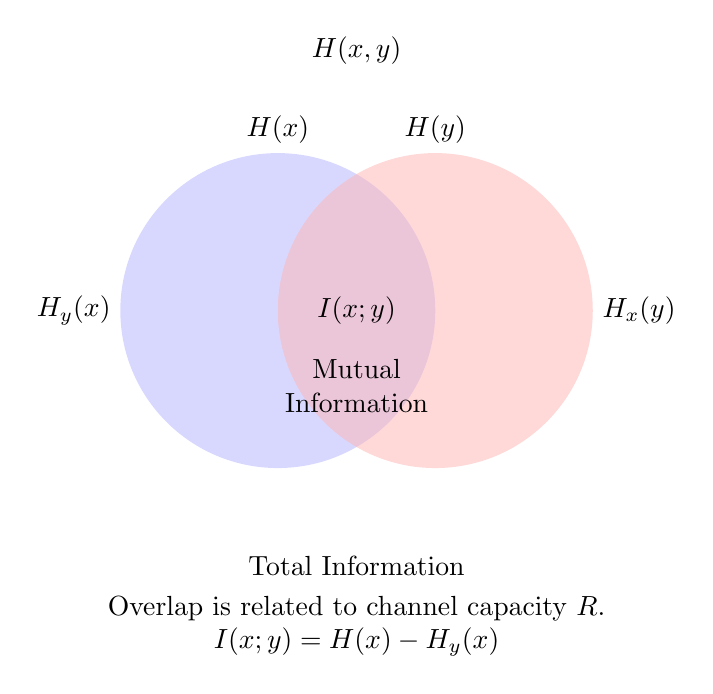
\begin{tikzpicture}
        % Define circle parameters
        \def\radius{2}
        \def\offset{1}

        % Draw the circles
        \begin{scope}
            \fill[blue!30, opacity=.5] (-\offset, 0) circle (\radius); % H(x) circle
            \fill[red!30, opacity=.5] (\offset, 0) circle (\radius); % H(y) circle
        \end{scope}

        % Add labels for the circles
        \node[above] at (-\offset, \radius) {$H(x)$};
        \node[above] at (\offset, \radius) {$H(y)$};

        % Add label for the intersection (Mutual Information)
        % Position this node in the overlap region
        \node (south) at (0, 0) {$I(x;y)$};
        \node[below=0.5cm of south, align=center] at (0,0) {Mutual\\Information};


        % Add label for H_y(x) (part of H(x) not overlapping H(y))
        % Position this node in the left crescent
        \node[left=0.5cm of {(-\radius-\offset+\offset/2, 0)}] {$H_y(x)$};


        % Add label for H_x(y) (part of H(y) not overlapping H(x))
        % Position this node in the right crescent
        \node[right=0.5cm of {(\radius+\offset-\offset/2, 0)}] {$H_x(y)$};

        % Add label for the union H(x,y)
        \node[above=0.5cm of {(0, \radius+\offset/2)}] {$H(x, y)$};
        \node[below=0.5cm of {(0, -\radius-\offset/2)}] {Total Information};

        % Add note about R
        \node[below=1cm of {(0, -\radius-\offset/2)}, align=center] {Overlap is related to channel capacity $R$. \\ $I(x;y) = H(x) - H_y(x)$};

    \end{tikzpicture}
    \caption{Venn diagram illustrating information theory concepts.}
    \label{fig:info_theory_venn}
\end{figure}

% \end{document}

You can visualize this with a Venn diagram:
\begin{itemize}
\item $H(x)$ is one circle (information in the transmitted signal).
\item $H(y)$ is another circle (information in the received signal).
\item $H(x, y)$ is the union of the circles (total information to describe both).
\item The overlap between the circles is the mutual information (information shared by $x$ and $y$).
\item $H_y(x)$ is the part of the $x$ circle that doesn't overlap with $y$.
\item $R$ is then the overlap, which you can calculate as the size of the $x$ circle minus the non-overlapping part.
\end{itemize}

These are all ways of saying the same thing: In a noisy channel, you don't get all the information you send. You only get the part that's reliably conveyed, and you have to subtract the uncertainty caused by the noise.

\begin{FormulaBox}
\[
H(X, Y) = H(X) + H(Y) - I(X; Y)
\]
\end{FormulaBox}

\begin{FormulaBox}
\[
I(X; Y) = H(X) - H(X \mid Y) = H(Y) - H(Y \mid X)
\]
\end{FormulaBox}

\begin{FormulaBox}
\[
H(X \mid Y) = H(X, Y) - H(Y)
\quad\quad
H(Y \mid X) = H(X, Y) - H(X)
\]
\end{FormulaBox}

\begin{tikzpicture}[
    node style/.style={draw, minimum width=2.6cm, minimum height=1cm, align=center}
  ]

  % Top row
  \node[node style] (joint)                      {$H(X, Y)$};

  % Middle row
  \node[node style, below=of joint] (hx)         {$H(X)$};
  \node[node style, right=2cm of hx] (hy)        {$H(Y)$};

  % Bottom row
  \node[node style, below=of hx] (hxgy)          {$H(X \mid Y)$};
  \node[node style, right=of hxgy] (ixy)         {$I(X; Y)$};
  \node[node style, right=of ixy] (hygx)         {$H(Y \mid X)$};

\end{tikzpicture}

% \documentclass{standalone}
% \begin{document}

% \documentclass{article}
% \usepackage{tikz}
% \usepackage{amsmath}
\usetikzlibrary{positioning, quotes}

% \begin{document}

\begin{figure}[h!]
    \centering
    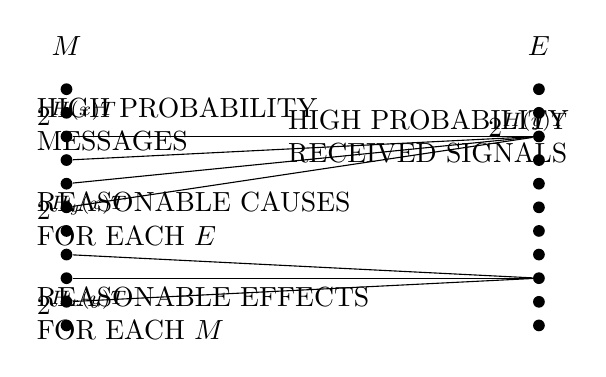
\begin{tikzpicture}[
        dot/.style={circle, fill, inner sep=1.5pt},
        text node/.style={align=left, anchor=west}
    ]

    % Define positions for the columns
    \def\mpos{0}
    \def\epos{6}
    \def\vsep{0.3} % Vertical separation between dots

    % Draw the M column (inputs)
    \node at (\mpos, 11*\vsep) [above] {$M$};
    \foreach \i in {0,...,10}
        \node[dot] (m\i) at (\mpos, \i*\vsep) {};

    % Draw the E column (outputs)
    \node at (\epos, 11*\vsep) [above] {$E$};
    \foreach \i in {0,...,10}
        \node[dot] (e\i) at (\epos, \i*\vsep) {};

    % Add labels and mathematical expressions on the left (M side)
    \node[text node] at (\mpos - 0.5, 9*\vsep) {$2^{H(x)T}$};
    \node[text node] at (\mpos - 0.5, 8.5*\vsep) {HIGH PROBABILITY\\MESSAGES};

    \node[text node] at (\mpos - 0.5, 5*\vsep) {$2^{H_y(x)T}$};
    \node[text node] at (\mpos - 0.5, 4.5*\vsep) {REASONABLE CAUSES\\FOR EACH $E$};

    \node[text node] at (\mpos - 0.5, 1*\vsep) {$2^{H_x(y)T}$};
    \node[text node] at (\mpos - 0.5, 0.5*\vsep) {REASONABLE EFFECTS\\FOR EACH $M$};


    % Add labels and mathematical expressions on the right (E side)
    \node[text node, anchor=east] at (\epos + 0.5, 8.5*\vsep) {$2^{H(y)T}$};
    \node[text node, anchor=east] at (\epos + 0.5, 8*\vsep) {HIGH PROBABILITY\\RECEIVED SIGNALS};


    % Draw the connecting lines
    % Approximate the connections based on the image
    \draw (m8) -- (e8);
    \draw (m7) -- (e8);
    \draw (m6) -- (e8);
    \draw (m5) -- (e8);

    \draw (m3) -- (e2);
    \draw (m2) -- (e2);
    \draw (m1) -- (e2);


    \end{tikzpicture}
    \caption{Schematic representation of the relations between inputs and outputs in a channel.}
    \label{fig:channel_relations}
\end{figure}

% \end{document}

\subsection*{Joint Entropy and Conditional Entropy}
% \setlength{\parindent}{0pt}
% \setlength{\parskip}{5pt}
% https://latex.org/forum/viewtopic.php?t=16729
% \renewcommand*{\thesubsubsection}{\arabic{subsubsection}} 

% \[
% P(x, y)
% \begin{array}{|c|cccc|}
% \cline{2-5}
% \multicolumn{1}{c|}{} & \multicolumn{4}{c|}{x} \\
% \cline{2-5}
% \multicolumn{1}{c|}{} & 1 & 2 & 3 & 4 \\
% \hline
% 1 & 1/8 & 1/16 & 1/32 & 1/32 \\
% y \quad 2 & 1/16 & 1/8 & 1/32 & 1/32 \\
% 3 & 1/16 & 1/16 & 1/16 & 1/16 \\
% 4 & 1/4 & 0 & 0 & 0 \\
% \hline
% \end{array}
% \]

% \documentclass{article}
% \usepackage{amsmath}
% \begin{document}
\renewcommand{\arraystretch}{1.15} % Adjust vertical spacing

% % P(x,y)
% \[
% \begin{array}{rc|cccc}
% \multicolumn{2}{c|}{P(x, y)} & \multicolumn{4}{c}{x} \\
%   &   & 1 & 2 & 3 & 4 \\
% \hline
%   & 1 & \sfrac{1}{8} & \sfrac{1}{16} & \sfrac{1}{32} & \sfrac{1}{32} \\
% y & 2 & \sfrac{1}{16} & \sfrac{1}{8} & \sfrac{1}{32} & \sfrac{1}{32} \\
%   & 3 & \sfrac{1}{16} & \sfrac{1}{16} & \sfrac{1}{16} & \sfrac{1}{16} \\
%   & 4 & \sfrac{1}{4} & 0 & 0 & 0 \\
% % \hline
% \end{array}
% \]

\href{https://docs.google.com/spreadsheets/d/1_JayV-shHoBeVebGs6C9hUGWOSVIkA8IjqfXhNity3E/edit?usp=sharing}{Link to Google sheets}
% same as the above, but add the marginal distributions
\begin{table}[h!]
    % \centering

\[
\begin{array}{rc|cccc|c}
\multicolumn{2}{c|}{\multirow{2}{*}{$P(x,y)$}} & \multicolumn{4}{c|}{x} & \multirow{2}{*}{$P(y)$} \\
  &   & 1 & 2 & 3 & 4 \\
\hline
\multirow{4}{*}{$y$} & 1 & \sfrac{1}{8} & \sfrac{1}{16} & \sfrac{1}{32} & \sfrac{1}{32} & \sfrac14 \\
  & 2 & \sfrac{1}{16} & \sfrac{1}{8} & \sfrac{1}{32} & \sfrac{1}{32} & \sfrac14 \\
  & 3 & \sfrac{1}{16} & \sfrac{1}{16} & \sfrac{1}{16} & \sfrac{1}{16} & \sfrac14 \\
  & 4 & \sfrac{1}{4} & 0 & 0 & 0 & \sfrac14 \\
\hline
\multicolumn{2}{c|}{P(x)} & \sfrac12 & \sfrac14 & \sfrac18 & \sfrac18
\end{array}
\]

    % \begin{tabular}{c|c}
    %      &  \\
    %      & 
    % \end{tabular}
    \caption{$P(x,y)$, $P(x)$ and $P(y)$}
    \label{tab:jointmarginal}
    
$P(x) : \text{tensor$^1$} = \sum_j P(x, y_j)$ 

$P(y) = \sum_i P(x_i, y)$

\end{table}

% P -> h
\begin{table}[h!]
% \begin{minipage}[t]{0.6\linewidth}
\[
\begin{array}{rc|cccc|c@{\hspace{3pt}}c}
\multicolumn{2}{c|}{\multirow{2}{*}{$h(x,y)$}} & \multicolumn{4}{c|}{x} & \multirow{2}{*}{$h(y)$} \\
  &   & 1 & 2 & 3 & 4 \\
\hline
\multirow{4}{*}{$y$} & 1 & \sfrac{3}{8} & \sfrac{4}{16} & \sfrac{5}{32} & \sfrac{5}{32} & \sfrac24 \\
  & 2 & \sfrac{4}{16} & \sfrac{3}{8} & \sfrac{5}{32} & \sfrac{5}{32} & \sfrac24 \\
  & 3 & \sfrac{4}{16} & \sfrac{4}{16} & \sfrac{4}{16} & \sfrac{4}{16} & \sfrac24 \\
  & 4 & \sfrac{2}{4} & 0 & 0 & 0 & \sfrac24 \\
\hline
% \multicolumn{2}{c|}{P(x)} & \sfrac12 & \sfrac14 & \sfrac18 & \sfrac18 \\
\multicolumn{2}{c|}{h(x)} & \sfrac12 & \sfrac24 & \sfrac38 & \sfrac38
\end{array}
\]
    \caption{$h(x,y)$, $h(x)$ and $h(y)$.}
    \label{tab:h_x}
% \end{minipage}
% \hfill
% \begin{minipage}[t]{0.4\linewidth}%\raggedright
% \end{minipage}
\[h(\cdot) = -p(\cdot)\log p(\cdot)\] % my formula
\end{table}

% P(X|Y)
% \begin{table}[h!]
\[
\begin{array}{rc|cccc|c@{\hspace{3pt}}c}
\multicolumn{2}{c|}{\multirow{2}{*}{$P(x\given y)$}} & \multicolumn{4}{c|}{x} & \multirow{2}{*}{$H(X\!\given y)$} \\
  &   & 1 & 2 & 3 & 4 \\
\hline
\multirow{4}{*}{$y$} & 1 & \sfrac{4}{8} & \sfrac{4}{16} & \sfrac{4}{32} & \sfrac{4}{32} & \sfrac74 \\
  & 2 & \sfrac{4}{16} & \sfrac{4}{8} & \sfrac{4}{32} & \sfrac{4}{32} & \sfrac74 \\
  & 3 & \sfrac{4}{16} & \sfrac{4}{16} & \sfrac{4}{16} & \sfrac{4}{16} & 2 \\
  & 4 & \sfrac{4}{4} & 0 & 0 & 0 & 0 \\
\hline
\multicolumn{7}{r}{H(X|Y)=\sfrac{11}8}
% \multicolumn{2}{c|}{P(x)} & \sfrac12 & \sfrac14 & \sfrac18 & \sfrac18 \\
% \multicolumn{2}{c|}{h(x)} & \sfrac12 & \sfrac24 & \sfrac38 & \sfrac38
\end{array}
\]
%     \caption{$h$}
%     \label{tab:h_x}
% \end{table}
$P(x\given y) = \frac{P(x,y)}{P(y)}$

\newpage
\section*{Non-symmetric channel example}

% \setlength{\floatsep}{0pt}
% \setlength{\textfloatsep}{0pt}
% \setlength{\intextsep}{0pt}

\begin{figure}[H]
\centering

% First subfigure: Joint Distribution
\begin{subfigure}[t]{0.4\textwidth}
\centering\vspace{0pt}
\[
\begin{array}{rc|cc|c}
\multicolumn{2}{c|}{\multirow{2}{*}{$P(x,y)$}} & \multicolumn{2}{c|}{x} & \multirow{2}{*}{$P(y)$} \\
 &   & 0 & 1 \\
\hline
\multirow{2}{*}{$y$} & 0 & 0.592 & 0.002 & 0.594 \\
 & 1 & 0.008 & 0.398 & 0.406 \\
\hline
\multicolumn{2}{c|}{P(x)} & 0.6 & 0.4
\end{array}
\]
% \vspace{-1em}
\[
H(X,Y) \approx \text{computed value}
\]
\caption{Joint Distribution and Joint Entropy}
\end{subfigure}
\hspace{-0.1cm}
% Second subfigure: Marginals and Entropy
\begin{subfigure}[t]{0.59\textwidth}
\centering\vspace{0pt}
% \[
% \begin{array}{c|c}
% x & P(x) \\
% \hline
% 0 & 0.6 \\
% 1 & 0.4
% \end{array}
% \qquad
% \begin{array}{c|c}
% y & P(y) \\
% \hline
% 0 & 0.594 \\
% 1 & 0.406
% \end{array}
% \vphantom{\begin{array}{c} A \\ B \\ C \\D\end{array}} % Same phantom height
% \]
% % \vspace{-1em}
% \[
% \begin{aligned}
% H(X) &= -0.6\log_2 0.6 - 0.4\log_2 0.4 \\
% H(Y) &= -0.594\log_2 0.594 - 0.406\log_2 0.406
% \end{aligned}
% \]
% \caption{Marginals and Entropy $H(X)$, $H(Y)$}

% \vspace{1.5em}
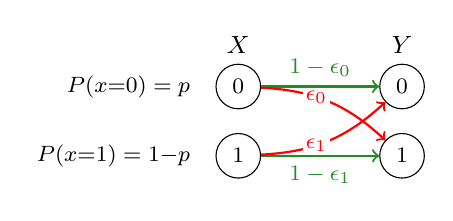
\begin{tikzpicture}[
  font=\footnotesize,
    node distance=.3cm,
    highlight/.style={fill=white, inner sep=1pt},
    state/.style={circle, draw, minimum size=.1cm},
    label/.style={above, font=\small}
]

% Nodes
\node[state] (X0) {$0$};
\node[state, right=1.5cm of X0] (Y0) {$0$};
\node[state, below=of X0] (X1) {$1$};
\node[state, right=1.5cm of X1] (Y1) {$1$};

% Labels
\node[label] at (X0.north) {$X$};
\node[label] at (Y0.north) {$Y$};

% Edges (correct transmissions)
\draw[->,ForestGreen,thick] (X0) -- node[above] {$1-\epsilon_0$} (Y0);
\draw[->,ForestGreen,thick] (X1) -- node[below] {$1-\epsilon_1$} (Y1);

% Edges (bit flips)
% \draw[->, thick, red] (X0) .. controls +(1,-0.5) and +(-1,-0.5) .. node[pos=.4, highlight] {$\epsilon_0$} (Y1);
% \draw[->, thick, red] (X1) .. controls +(1,0.5) and +(-1,0.5) .. node[pos=.4, highlight] {$\epsilon_1$} (Y0);

% Upper arrow: Downward arc using bend left
\draw[->, thick, red, bend left=20] 
    (X0) to node[pos=.4, highlight] {$\epsilon_0$} (Y1);

% Lower arrow: Upward arc using bend right
\draw[->, thick, red, bend right=20] 
    (X1) to node[pos=.4, highlight] {$\epsilon_1$} (Y0);

% Input probabilities
\node[left=0.2cm of X0] {$P(x{=}0)=p$};
\node[left=0.2cm of X1] {$P(x{=}1)=1{-}p$};

\end{tikzpicture}
\[
\begin{aligned}
\epsilon_0&=P(Y{=}1\given X{=}0)=0.008/0.6=1.3\% \\
\epsilon_1&=P(Y{=}0\given X{=}1)=0.002/0.4=0.5\%   
\end{aligned}
\]
% \vspace{1.5em}
\caption{Non-symmetric error probabilities}
\label{fig:bsc}
\end{subfigure}

\end{figure}

\begin{figure}[h!]\centering
  \begin{subfigure}{0.45\textwidth}\centering
\[
\begin{array}{rc|cc|c}
\multicolumn{2}{c|}{\multirow{2}{*}{$P(x,y)$}} & \multicolumn{2}{c|}{x} & \multirow{2}{*}{$P(y)$} \\
  &   & 0 & 1 \\
\hline
\multirow{2}{*}{$y$}  & 0 & 0.592 & 0.002 & 0.594 \\
 & 1 & 0.008 & 0.398 & 0.406 \\
\hline
\multicolumn{2}{c|}{P(x)} & 0.6 & 0.4
\end{array}
\]
\caption{$P(x,y)$, $P(x)$ and $P(y)$}
\label{tab:nonsymmprob}
  \end{subfigure}
% \hfill
\hspace{-0.4cm}
  \begin{subfigure}{0.45\textwidth}\centering
\[
\begin{array}{rc|cc|c}
\multicolumn{2}{c|}{\multirow{2}{*}{$P(x,y)$}} & \multicolumn{2}{c|}{x} & \multirow{2}{*}{$P(y)$} \\
  &   & 0 & 1 \\
\hline
\multirow{2}{*}{$y$}  & 0 & 0.592 & 0.002 & 0.594 \\
 & 1 & 0.008 & 0.398 & 0.406 \\
\hline
\multicolumn{2}{c|}{P(x)} & 0.6 & 0.4
\end{array}
\]
\caption{$P(x,y)$, $P(x)$ and $P(y)$}
\label{tab:nonsymmprob}
  \end{subfigure}

    % \begin{tabular}{c|c}
    %      &  \\
    %      & 
    % \end{tabular}
\end{figure}
% \bigskip

\begin{figure}[htbp!]
\centering
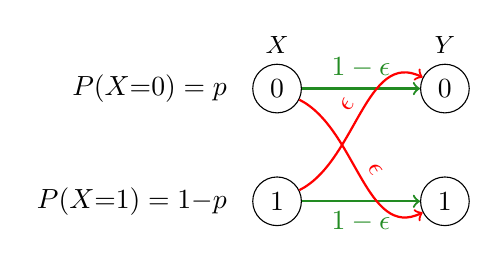
\begin{tikzpicture}[
    node distance=.8cm,
    state/.style={circle, draw, minimum size=.1cm},
    label/.style={above, font=\small}
]

% Nodes
\node[state] (X0) {$0$};
\node[state, right=1.5cm of X0] (Y0) {$0$};
\node[state, below=of X0] (X1) {$1$};
\node[state, right=1.5cm of X1] (Y1) {$1$};

% Labels
\node[label] at (X0.north) {$X$};
\node[label] at (Y0.north) {$Y$};

% Edges (correct transmissions)
\draw[->,ForestGreen,thick] (X0) -- node[above] {$1-\epsilon$} (Y0);
\draw[->,ForestGreen,thick] (X1) -- node[below] {$1-\epsilon$} (Y1);

% Edges (bit flips)
\draw[->, thick, red] (X0) .. controls +(1,-0.5) and +(-1,-0.5) .. node[midway, sloped, above] {$\epsilon$} (Y1);
\draw[->, thick, red] (X1) .. controls +(1,0.5) and +(-1,0.5) .. node[midway, sloped, above] {$\epsilon$} (Y0);

% Input probabilities
\node[left=0.2cm of X0] {$P(X{=}0)=p$};
\node[left=0.2cm of X1] {$P(X{=}1)=1{-}p$};

\end{tikzpicture}
\caption{Binary symmetric channel}
\label{fig:bsc}
\end{figure}

\penalty-100
% \pagebreak
% \clearpage
% \newpage
Total error $=\sum_{x\neq y} P(x, y)=0.008+0.002=1\%$.

% Given what you observed/received, what was most likely transmitted ($\ldots$ chance 0 was transmitted and $\ldots$ chance 1 was transmitted).
\begin{description}
\item[\normalfont Given $\text{received}{=}0$,]
\begin{multline*}    
P(\text{transmitted}{=}0\given\text{received}{=}0)=P(T{=}0,R{=}0)/P(R{=}0)\\
=0.592/0.594=0.997
\end{multline*}
\begin{multline*}    
P(\text{transmitted}{=}1\given\text{received}{=}0)=P(T{=}1,R{=}0)/P(R{=}0)\\
=0.002/0.594=0.003
\end{multline*}

\item[\normalfont Given $\text{received}{=}1$,]
\begin{multline*}    
P(\text{transmitted}{=}0\given\text{received}{=}1)=P(T{=}0,R{=}1)/P(R{=}1)\\
=0.008/0.406=0.020
\end{multline*}
\begin{multline*}    
P(\text{transmitted}{=}1\given\text{received}{=}1)=P(T{=}1,R{=}1)/P(R{=}1)\\
=0.398/0.406=0.980
\end{multline*}
\end{description}

Interpretation:
\begin{itemize}
    \item If you received a $0$, there's a 99.7\% chance a $0$ was transmitted, 0.3\% chance a $1$ was transmitted.
    \item If you received a $1$, there's a 98\% chance a $1$ was transmitted. 2\% chance a $0$ was transmitted.
\end{itemize}


% \penalty=-100
% \newpage

\begin{thebibliography}{9}
\bibitem{itprimer} Thomas D. Schneider. \textit{Information Theory Primer}. April 2007.
\bibitem{shannon} Shannon, C. E. (1948) A mathematical theory of communication.
\textit{Bell Sys.\ Tech.\ J.} 379-423, 623-656.
% \bibitem{einstein} Albert Einstein. \textit{Zur Elektrodynamik bewegter K{\"o}rper}. (German) [\textit{On the electrodynamics of moving bodies}]. Annalen der Physik, 322(10):891–921, 1905.
% \bibitem{knuthwebsite} Knuth: Computers and Typesetting,\\\texttt{http://www-cs-faculty.stanford.edu/\~{}uno/abcde.html}
\end{thebibliography}
\end{document}
